\documentclass[11pt]{extbook}
\renewcommand{\baselinestretch}{1.04}

\usepackage{verbatim} % For comments

\usepackage[dutch,british]{babel}

% for booklet
%\usepackage[paperheight=240mm,paperwidth=170mm,top=20mm,bottom=20mm,right=20mm,left=20mm]{geometry}
%\usepackage[height=250mm,width=180mm,cam,noinfo,pdftex,center]{crop}

%%%% Things I did for reading version%%%%%%%%%%%%
\usepackage[paperheight=297mm,paperwidth=210mm,top=25mm,bottom=25mm,right=25mm,left=25mm]{geometry}
%\usepackage{pdfpages}
%%%%%%%%%%%%%%%%%%


\usepackage{nameref}
\usepackage[hypertexnames=false,hidelinks,bookmarks]{hyperref}

\usepackage{etoolbox}
% Fix multiple links for references issue.
\makeatletter
\pretocmd{\NAT@citex}{%
  \let\NAT@hyper@\NAT@hyper@citex
  \def\NAT@postnote{#2}%
  \setcounter{NAT@total@cites}{0}%
  \setcounter{NAT@count@cites}{0}%
  \forcsvlist{\stepcounter{NAT@total@cites}\@gobble}{#3}}{}{}
\newcounter{NAT@total@cites}
\newcounter{NAT@count@cites}
\def\NAT@postnote{}

% include postnote and \citet closing bracket in hyperlink
\def\NAT@hyper@citex#1{%
  \stepcounter{NAT@count@cites}%
  \hyper@natlinkstart{\@citeb\@extra@b@citeb}#1%
  \ifnumequal{\value{NAT@count@cites}}{\value{NAT@total@cites}}
    {\ifNAT@swa\else\if*\NAT@postnote*\else%
     \NAT@cmt\NAT@postnote\global\def\NAT@postnote{}\fi\fi}{}%
  \ifNAT@swa\else\if\relax\NAT@date\relax
  \else\NAT@@close\global\let\NAT@nm\@empty\fi\fi% avoid compact citations
  \hyper@natlinkend}
\renewcommand\hyper@natlinkbreak[2]{#1}

% avoid extraneous postnotes, closing brackets
\patchcmd{\NAT@citex}
  {\ifNAT@swa\else\if*#2*\else\NAT@cmt#2\fi
   \if\relax\NAT@date\relax\else\NAT@@close\fi\fi}{}{}{}
\patchcmd{\NAT@citex}
  {\if\relax\NAT@date\relax\NAT@def@citea\else\NAT@def@citea@close\fi}
  {\if\relax\NAT@date\relax\NAT@def@citea\else\NAT@def@citea@space\fi}{}{}
\makeatother

\usepackage{graphicx}
\usepackage{longtable}
\usepackage{tabularx}
\usepackage{floatrow}
\DeclareFloatSeparators{captionmargin}{\hspace{2.5mm}} 
\usepackage{adjustbox}
\usepackage{float}
\floatstyle{plaintop}
\restylefloat{table}
\usepackage{pbox}
\usepackage{wrapfig}
\setlength{\textfloatsep}{16pt}
\setlength{\intextsep}{16pt}
\renewcommand{\bottomfraction}{0.7}
\usepackage[ansinew]{inputenc}

\usepackage{multirow}
\usepackage{booktabs}
%\usepackage{placeins}

% Symbol packages
\usepackage[fleqn]{amsmath}
\usepackage{amssymb}
\usepackage{upgreek}
\usepackage{bm}
\usepackage{mathtools}
\usepackage{nccmath}
\usepackage{array}   % for \newcolumntype macro
\newcolumntype{L}{>{$}l<{$}} % math-mode version of "l" column type
\newcolumntype{C}{>{$}c<{$}} % math-mode version of "l" column type

% Set fonts.
\usepackage{ebgaramond}
\usepackage{uarial}
\usepackage[T1]{fontenc}
\newcommand{\fakebf}{\fontfamily{mdugm}\fontseries{b}\selectfont\small}
\DeclareTextFontCommand{\textbf}{\fakebf}

% landscape package
\usepackage{lscape}

% Set captions and section title fonts.
\usepackage[tableposition=top]{caption}
% Declare sans-serif math version for the captions.
\DeclareMathVersion{captionmath}
\SetSymbolFont{operators}{captionmath}{OT1}{cmbr}{m}{n}
\SetSymbolFont{letters}{captionmath}{OML}{cmbrm}{m}{it}
\SetSymbolFont{symbols}{captionmath}{OMS}{cmbrs}{m}{n}
\SetMathAlphabet\mathbf{captionmath}{OT1}{cmbr}{bx}{n}
\SetMathAlphabet\mathsf{captionmath}{OT1}{cmbr}{m}{n}
\SetMathAlphabet\mathit{captionmath}{OT1}{cmbr}{m}{it}
\SetMathAlphabet\mathtt{captionmath}{OT1}{cmtl}{m}{n}
\DeclareCaptionFont{sansmath}{\mathversion{captionmath}}

%%%%%%%%%%%%%%%%%%%%%%%%%%%%%%%%%%%%%%%%%%%%%%%%%
% Glossaries for list of symbols
\usepackage[symbols,nogroupskip,nonumberlist,automake]{glossaries-extra}
\makeglossaries

\setlength{\glsdescwidth}{0.8\linewidth}
\glsxtrnewsymbol[description={Front-to-back translatory optic flow in a free-flight (s$^{-1}$)}]{tof}{\ensuremath{T_{OF}}}
\glsxtrnewsymbol[description={Set-point of front-to-back translatory optic flow in a free-flight (s$^{-1}$)}]{tofs}{\ensuremath{T^*_{OF}}}
\glsxtrnewsymbol[description={Flight speed in a free-flight condition (m s$^{-1}$)}]{vf}{\ensuremath{V_F}}
\glsxtrnewsymbol[description={Distance from the surface in a free-flight condition (m)}]{D}{\ensuremath{D}}
\glsxtrnewsymbol[description={Time-to-touchdown (s)}]{t}{\ensuremath{t}}
\glsxtrnewsymbol[description={Fit percentage}]{F}{\ensuremath{F}}
\glsxtrnewsymbol[description={Coefficient of determination}]{R2}{\ensuremath{R^2}}
\glsxtrnewsymbol[description={Time-to-contact parameter (s) (inverse of optical expansion rate $r$)}]{tau}{\ensuremath{\tau}}

\glsxtrnewsymbol[description={Time-to-contact-rate (time derivative of time-to-contact $r$)}]{taudot}{\ensuremath{\dot{\tau}}}
\glsxtrnewsymbol[description={Relative rate of expansion or optical expansion rate (s$^{-1}$)}]{r}{\ensuremath{r}}
\glsxtrnewsymbol[description={Optical expansion rate at the start of the entry segment (s$^{-1}$)}]{r0}{\ensuremath{r_0}}
\glsxtrnewsymbol[description={Initial distance from the landing platform at which the entry segment starts (m)}]{y0}{\ensuremath{y_0}}
\glsxtrnewsymbol[description={Average approach acceleration $A$ during an entry segment (m s$^{-2}$)}]{Ameane}{\ensuremath{\overline{A}_{e}}}
\glsxtrnewsymbol[description={Average airspeed $U_A$ during an entry segment (m s$^{-1}$)}]{UAe}{\ensuremath{\overline{U}_{A~e}}}
\glsxtrnewsymbol[description={Change in approach velocity during an entry segment (m s$^{-1}$)}]{deltaV}{\ensuremath{\Delta V}}
\glsxtrnewsymbol[description={Time duration of an entry segment (s)}]{deltat}{\ensuremath{\Delta t}}
\glsxtrnewsymbol[description={Optical expansion acceleration; calculated as time derivative of optical expansion rate (s$^{-2}$)}]{rdot}{\ensuremath{\dot{r}}}
\glsxtrnewsymbol[description={Estimate of optical expansion acceleration in an entry segment (s$^{-2}$)}]{rdote}{\ensuremath{\dot{r}_e}}
\glsxtrnewsymbol[description={Step-change of optical expansion rate required in an entry segment (s$^{-1}$)}]{deltare}{\ensuremath{\Delta r_e}}
\glsxtrnewsymbol[description={Temporal variation of relative rate of expansion in a combined pair of constant-$r$ and entry segments (s$^{-1}$)}]{rct}{\ensuremath{r_c(t)}}
\glsxtrnewsymbol[description={Low-pass filtered temporal variation of relative rate of expansion in a combined pair of constant-$r$ and entry segments (s$^{-1}$)}]{rft}{\ensuremath{r_f(t)}}
\glsxtrnewsymbol[description={Temporal variation of relative rate of expansion in a combined pair of constant-$r$ and entry segments obtained after simulating a transfer function (s$^{-1}$)}]{rst}{\ensuremath{r_s(t)}}
\glsxtrnewsymbol[description={Set-point of relative rate of expansion or optical expansion rate; mean value of optical expansion rate in a constant-$r$ segment  (s$^{-1}$)}]{rs}{\ensuremath{r^*}}
\glsxtrnewsymbol[description={Switch-reversal set-point of optical expansion rate (s$^{-1}$)}]{srs}{\ensuremath{r_0^*}}
\glsxtrnewsymbol[description={Slope of linear relationship between the logarithmic transformations of the set-points of optical expansion rate $r^*$ and the mean distance to the surface $y^*$; a parameter similar to time-to-contact rate $\dot{\tau}$}]{m}{\ensuremath{m}}
\glsxtrnewsymbol[description={Change in set-point of optical expansion rate between two consecutive constant-$r$ segments in a landing approach (s$^{-1}$)}]{deltars}{\ensuremath{\Delta r^*}}
\glsxtrnewsymbol[description={Mean value of distance to the surface in a constant-$r$ segment  (m)}]{ys}{\ensuremath{y^*}}
\glsxtrnewsymbol[description={Time duration during a constant-$r$ segment  (s)}]{ts}{\ensuremath{\Delta t^*}}
\glsxtrnewsymbol[description={Mean value of approach acceleration $A$ in a constant-$r$ segment  (m s$^{-2}$)}]{As}{\ensuremath{A^*}}
\glsxtrnewsymbol[description={Mean value of approach velocity $V$ in a constant-$r$ segment  (m s$^{-1}$)}]{Vs}{\ensuremath{V^*}}
\glsxtrnewsymbol[description={An axis of a landing platform coordinate system; defined in a direction normal to the landing platform (m)}]{y}{\ensuremath{y}}
\glsxtrnewsymbol[description={An axis of a landing platform coordinate system; defined in a plane parallel to the ground (m)}]{x}{\ensuremath{x}}
\glsxtrnewsymbol[description={An axis of a landing platform coordinate system; defined in a vertically up direction (m)}]{z}{\ensuremath{z}}
\glsxtrnewsymbol[description={Approach velocity towards the landing platform (m s$^{-1}$)}]{V}{\ensuremath{V}}
\glsxtrnewsymbol[description={Approach acceleration towards the landing platform (m s$^{-2}$)}]{A}{\ensuremath{A}}
\glsxtrnewsymbol[description={Three-dimensional speed at the start of the landing maneuver (m s$^{-1}$)}]{Ustart}{\ensuremath{U_{start}}}
\glsxtrnewsymbol[description={Average flight speed between two consecutive constant-$r$ segments for a hybrid landing strategy (m s$^{-1}$)}]{UH}{\ensuremath{U_{H}}}
\glsxtrnewsymbol[description={Average flight speed between two consecutive constant-$r$ segments for a constant-$r$ landing strategy (m s$^{-1}$)}]{Ur}{\ensuremath{U_{r}}}
\glsxtrnewsymbol[description={Average flight speed between two consecutive constant-$r$ segments for a constant-$\dot{\tau}$ landing strategy (m s$^{-1}$)}]{Utaudot}{\ensuremath{U_{\dot{\tau}}}}
\glsxtrnewsymbol[description={Displacement normal to the landing surface during a constant-$r$ segment (m)}]{deltay1}{\ensuremath{\Delta y_1} or \ensuremath{\Delta y^*}}
\glsxtrnewsymbol[description={Displacement normal to the landing surface for a set of consecutive constant-$r$ segments (m)}]{deltay2}{\ensuremath{\Delta y_2}}
\glsxtrnewsymbol[description={Threshold factor used in the set-point extraction algorithm}]{f}{\ensuremath{f}}
\glsxtrnewsymbol[description={Space-time array ($x,y,z,t$)}]{vecX}{\ensuremath{\bm{X}}}
\glsxtrnewsymbol[description={Ground-velocity vector ($u,v,w$) or ($u_G,v_G,w_G$) in landing platform coordinate system (m s$^{-1}$)}]{vecU}{\ensuremath{\bm{U}} or \ensuremath{\bm{U_G}}}
\glsxtrnewsymbol[description={Wind-velocity vector ($u_W,0,0$) in landing platform coordinate system (m s$^{-1}$)}]{vecUW}{\ensuremath{\bm{U_W}}}
\glsxtrnewsymbol[description={Air-velocity vector ($u_A,v_A,w_A$) in landing platform coordinate system (m s$^{-1}$)}]{vecUA}{\ensuremath{\bm{U_A}}}
\glsxtrnewsymbol[description={Acceleration vector ($a_x,a_y,a_z$) (m s$^{-2}$)}]{vecA}{\ensuremath{\bm{A}}}
\glsxtrnewsymbol[description={Parameters of a gamma distribution}]{ab}{\ensuremath{a,~b}}
\glsxtrnewsymbol[description={Probability of a bumblebee exhibiting low approach velocity phase}]{PlowV}{\ensuremath{P_{\textrm{low }V}}}
%%%%%%%%%%%%%%%%%%%%%%%%%%%%%%%%%%%%%%%%%%%%%%%%%

\captionsetup{figurename=Figure,font={scriptsize,sf,sansmath},labelfont=bf}

% Make sure equation labels are always normal size, even if the equations themselves are smaller.
\makeatletter
\def\maketag@@@#1{\hbox{\m@th\normalfont\normalsize#1}}
\makeatother

% Format headings.
\usepackage[noindentafter]{titlesec}
% Fix bug
\makeatletter
\patchcmd{\ttlh@hang}{\parindent\z@}{\parindent\z@\leavevmode}{}{}
\patchcmd{\ttlh@hang}{\noindent}{}{}{}
\makeatother
\titleformat{\chapter}{\vspace{-50pt}\Huge}{\thechapter}{4mm}{\Huge\vspace{-30pt}}

\titleformat{\section}{\normalfont\sffamily\Large\bfseries}{\thesection}{4mm}{}
\titlespacing{\section}{0pt}{11pt plus 6pt minus 2pt}{6pt plus 0pt minus 0pt}
\titleformat{\subsection}{\normalfont\sffamily\large\bfseries}{\thesubsection}{3mm}{}
\titlespacing{\section}{0pt}{8pt plus 4pt minus 2pt}{6pt plus 0pt minus 0pt}
\titleformat{\subsubsection}{\normalfont\sffamily\normalsize\bfseries}{\thesubsubsection}{3mm}{}
\titlespacing{\section}{0pt}{8pt plus 4pt minus 2pt}{6pt plus 0pt minus 0pt}

% Define \thumb command for use in the header
\usepackage{tikz}
\usetikzlibrary{calc}
\usepackage{xcolor}

\newcommand{\thumb}[2]{%
\begin{tikzpicture}[remember picture,overlay]
\fill[fill=lightgray]
($(current page.north east) + (-10mm,-5mm) + (0,#2mm)$) 
-- ($(current page.north east) + (5mm,-5mm) + (0,#2mm)$)
-- ($(current page.north east) + (5mm,5mm) + (0,#2mm)$)
-- ($(current page.north east) + (-10mm, 5mm) + (0,#2mm)$)
-- cycle;
\node(test) at ($(current page.north east) + (-5mm,#2mm)$){\Huge\textcolor{white}{#1}};
\end{tikzpicture}}

% Fish flickbook
\newcommand{\fish}{%
\begin{tikzpicture}[remember picture,overlay]
\node(test) at ($(current page.north west) + (10mm,-120mm)$){\includegraphics[width=20mm]{figures/flickbook/frame\thepage}};
\end{tikzpicture}}
%\renewcommand{\fish}{\textit{fish \thepage}}

% Title page
\newcommand{\titleimage}[1]{%
\begin{tikzpicture}[remember picture,overlay]
\node(test) at ($(current page.center)$){\includegraphics[width=180mm]{#1}};
\end{tikzpicture}}

% Customise headers and footers
\usepackage{fancyhdr}

\fancypagestyle{fishempty}{%
\fancyhf{}
\fancyhead[LE]{\fish}
\renewcommand{\headrulewidth}{0pt}
}

\pagestyle{fancy}

\fancyhf{}
\fancyfoot[LE,RO]{\thepage}

%%%% Things I did for reading version%%%%%%%%%% remove them for final version
%\fancyfootoffset{2.5cm}
%%%%%%%%%%%%%%%%%%%%%%%%%%%%%%%%%%%%%%%%%%%%%%%%%%

\newcommand{\chapterthumb}{}
%\newcommand{\chapterthumb}{placeholder for page thumbs}
\fancyhead[CO]{\chapterthumb}
%\fancyhead[LE]{\fish}
\renewcommand{\headrulewidth}{0pt}

\makeatletter
\let\ps@plain\ps@fancy
\makeatother

\makeatletter
\newcommand{\cleardoublepageeven}{\clearpage\if@twoside\ifodd\c@page \hbox{}\newpage\if@twocolumn\hbox{}\newpage\fi\fi\fi}
\makeatother

% Remove chapter heading for chapters with a (manually defined) title page - these will be added manually later.
\makeatletter
\newcommand{\unchapter}[1]{%
  \begingroup
  %\let\ps@plain\ps@empty
  %\let\ps@fancy\ps@empty
  \renewcommand{\cleardoublepage}{\cleardoublepageeven}
  \let\@makechapterhead\@gobble % make \@makechapterhead do nothing
  \chapter{#1}
  \endgroup
}
\makeatother

% Make fake chapter heading for the pageref in the TOC, so we can insert empty pages for the title page.
\makeatletter
\newcommand{\chapterpagemark}[1]{%
  \begingroup
  %\let\ps@plain\ps@empty
  %\let\ps@fancy\ps@empty
  % Make sure our chapters start at the even page by redefining \cleardoublepage, which is used in the macro @makechapterhead.
  \renewcommand{\cleardoublepage}{\cleardoublepageeven}
  \let\@makechapterhead\@gobble % make \@makechapterhead do nothing
  \chapter{#1}
  \addtocounter{chapter}{-1}
  \endgroup
}
\makeatother

% Formatting commands to use in text.
\newcommand{\figuretitle}[1]{{\bfseries #1}}
\newcommand{\latin}{\textit}
\newcommand{\chapterref}[2]{\mbox{\hyperref[#1]{\textbf{#2}}}}
\newcommand{\code}[1]{{\tt #1}}

% Bibliography
\usepackage[sectionbib]{natbib}
\usepackage{bibunits}
\defaultbibliographystyle{jxb_links}
\defaultbibliography{library}
\setlength{\bibsep}{1.2mm}
\addto{\captionsbritish}{\renewcommand{\bibname}{References}}

% Math and text commands.
\newcommand{\bmvec}[1]{\bm{\mathrm{#1}}}
\newcommand{\swimming}{\mathrm{Sw}}
\newcommand{\reynolds}{\mathrm{Re}}
\newcommand{\strouhal}{\mathrm{St}}
\newcommand{\CoT}{\mathrm{CoT}}
\renewcommand{\d}{\mathrm{d}}
\newcommand{\T}{\mathrm{T}}
\newcommand{\deriv}[2]{\frac{\d #1}{\d #2}}
\newcommand{\derivn}[3]{\frac{\d^#3 #1}{\d #2^#3}}
\newcommand{\pderiv}[2]{\frac{\partial #1}{\partial #2}}
\newcommand{\pderivn}[3]{\frac{\partial^#3 #1}{\partial #2^#3}}
\newcommand{\ci}{CI$_\textrm{95\%}$}
\newcommand{\scinum}[2]{#1~\cdot~10^{#2}}
\newcommand{\dimension}{\mathsf}



% Make sure paragraphs stay together - sometimes they are stretched apart automatically.
\setlength{\parskip}{2pt}

\begin{document}
\bibliographyunit[\chapter]


\chapter*{Supplemental information}
\renewcommand{\thesection}{S\arabic{section}}
\renewcommand{\thesubsection}{S\arabic{section}.\arabic{subsection}}
\renewcommand{\thesubsubsection}{S\arabic{section}.\arabic{subsection}.\arabic{subsubsection}}
\renewcommand{\theequation}{S\arabic{equation}}
\renewcommand{\thefigure}{S\arabic{figure}}
\renewcommand{\thetable}{S\arabic{table}}
\setcounter{section}{0}
\setcounter{subsection}{0}
\setcounter{equation}{0}
\setcounter{figure}{0}
\setcounter{table}{0}

\vspace*{3cm}
{\huge Bumblebees actively compensate for the adverse effects of steady sidewinds during visually guided landings}
\\*[0.5cm]
{\large Pulkit Goyal, Johan L. van Leeuwen, Florian T. Muijres}
\clearpage

\section{Figures}
\label{section_sw_s_figures}

\begin{figure}[H]
	\centering
	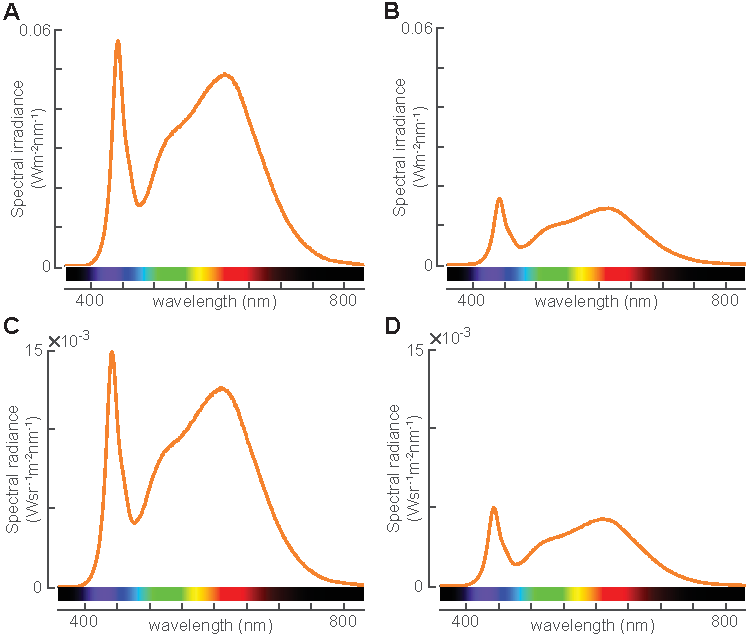
\includegraphics{figures/chapter4/figure_sw_s_lightintensity}
	\caption{\figuretitle{Light spectrum used in the experiments}. Spectral irradiance (A) and spectral radiance (C) at the center of the flight arena. Spectral irradiance (B) and spectral radiance (D) at the centre of the landing platforms.}
	\label{figure_sw_s_lightintensity}
\end{figure}

\newpage
\begin{figure}[H]
	\centering
	\includegraphics[scale=0.95]{figures/chapter4/figure_sw_s02_logrref_vs_y}
	\caption{\figuretitle{The variation of set-point of optical expansion rate $\boldsymbol{r^*}$ with distance to the surface $\boldsymbol{y^*}$ in the logarithmic domain as identified by the linear mixed-effects model in Equation~\ref{eq:sw_model_per_track} (Table~\ref{tb:sw_model_per_track}).}}
	\label{figure_sw_s02_logrref_vs_y}
\end{figure}

\newpage
\begin{figure}[H]
	\centering
	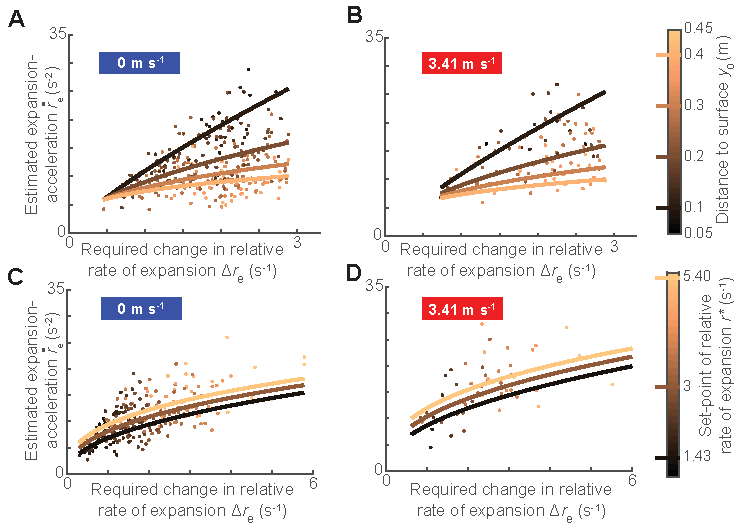
\includegraphics[scale=0.95]{figures/chapter4/figure_sw_s03_rdot}
	\caption{\figuretitle{The variation of optical expansion-acceleration $\boldsymbol{\dot{r}_e}$ with explanatory variables as identified by the linear mixed-effects model in Equation~\ref{eq:sw_rdot_amean_model} (Table~\ref{tb:sw_rdot_model}).} (A,B) The variation of expansion-acceleration $\dot{r}_e$ due to the interaction between the required step-change in relative rate of expansion ($\Delta r_e$) and the starting distance of the entry segment from the landing surface ($y_0$) in still air (A) and fastest tested wind speed (B). (C,D) The variation of expansion-acceleration $\dot{r}_e$ due to the interaction between the required step-change in relative rate of expansion ($\Delta r_e$) and the final set-point to reach ($r^*$) in an entry segment for still air (C) and fastest tested wind speed (D). (A,B) The curves depict the statistical model output at the median value $r^*=2.98~ s^{-1}$, and data points are shown for the interval $r^* \in [2.48,~3.48]~s^{-1}$. (C,D) The curves depict the statistical model output at the median value $y_0=0.28~m$, and data points are shown for the interval $y_0 \in [0.255,~0.305]~m$.  }
	\label{figure_sw_s03_rdot}
\end{figure}

\section{Tables}
\label{section_sw_s_tables}

\begin{landscape}
	\begin{table}\centering
		\captionsetup{width=0.7\textwidth, justification=justified}
		\caption{\figuretitle{Pseudo-random treatment schedule followed during experiments to record the landing maneuvers of bumblebees in different steady sidewinds.}}
		\label{tb:swind_treatment_schedule}
		
			\begin{tabular}{CCCCCCCCCCCCC}
				\toprule
				\multicolumn{2}{c}{Time (hours)} & \multicolumn{11}{c}{Days}     \\
				\cmidrule(lr){1-2} \cmidrule(lr){3-13}\\
				\textrm{start}       & \textrm{end} & 1  & 2  & 3  & 4  & 5  & 6  & 7  & 8  & 9  & 10 & 11  \\
				\midrule \\ 
				\\
				80000  & 93000  & u_{w3}^* & u_{w2} & u_{w4} & u_{w0} & u_{w5} & u_{w1} & u_{w2} & u_{w4} & u_{w3} & u_{w5} & u_{w2}^* \\
				93000  & 110000 & u_{w5} & u_{w1} & u_{w2} & u_{w3} & u_{w4} & u_{w0} & u_{w5} & u_{w1} & u_{w2} & u_{w4} & u_{w1}^* \\
				110000 & 123000 & u_{w1} & u_{w5} & u_{w0} & u_{w4} & u_{w3} & u_{w2} & u_{w0} & u_{w3} & u_{w4} & u_{w1} & u_{w4}^* \\
				123000 & 140000 & u_{w4} & u_{w0} & u_{w5} & u_{w2} & u_{w1} & u_{w3} & u_{w4} & u_{w5} & u_{w0} & u_{w2} & u_{w5} \\
				140000 & 153000 & u_{w2} & u_{w4} & u_{w3} & u_{w1} & u_{w0} & u_{w5} & u_{w3} & u_{w2} & u_{w1} & u_{w0} & u_{w3} \\
				153000 & 170000 & u_{w0}^* & u_{w3} & u_{w1} & u_{w5} & u_{w2}^* & u_{w4} & u_{w1}^* & u_{w0} & u_{w5} & u_{w3} & u_{w0} \\
				
				\\
				\multicolumn{13}{l}{\scriptsize{*During these treatments, the wind speed could not be measured using the hot-wire anemometer.}} \\
				\multicolumn{13}{l}{\scriptsize{Wind speeds in $m\,s^{-1}$: $u_{w0} = 0$, $u_{w1} = 0.28$, $u_{w2} = 0.98$, $u_{w3} = 1.77$, $u_{w4} = 2.54$, $u_{w5} = 3.41$}} \\
				\bottomrule 
			\end{tabular}
	\end{table}
\end{landscape}
\clearpage


\begin{table}[H]\centering
	\captionsetup{width=\textwidth, justification=justified}
	\caption{\figuretitle{The analysis of landing frequency of bumblebees in different wind speeds}. The post-hoc tests compare differences between the number of landings per hour $N$ in different wind conditions (statistical model as given by Equation~\ref{eq:sw_model_N}: 
		$ N_{\textrm{takeoff},i,d,t} \text{ or } N_{\textrm{freeflight},i,d,t} \sim N( \alpha_0 + \alpha_d + \alpha_t + \sum_{j=1}^{5} \beta_j~\textrm{WIND}_{j,i,d,t},~\sigma^2)$).}
	\label{tb:sw_model_N}
	\begin{tabular}{p{3.5cm}LLLL}
		Effect on $N_{\textrm{freeflight},i,d,t}$            & &   & & \\
		\toprule
		\toprule
		Fixed effect             & \text{Estimate} & \text{Std error} & \text{t value} & \text{Pr(\textgreater{}|t|)} \\
		\midrule
			$\alpha$ & 280.83  & 28.22 & 9.95  & 8.34E-09 \\
		$\beta_1$&  -69.41  & 22.47 & -3.09 & 0.0038   \\
		$\beta_2$& -94.72  & 22.68 & -4.18 & 0.0002   \\
		$\beta_3$& -135.19 & 21.44 & -6.31 & 2.48E-07 \\
		$\beta_4$& -165.55 & 21.79 & -7.60 & 4.31E-09 \\
		$\beta_5$& -168.61 & 21.17 & -7.97 & 1.4E-09 \\
		
		& &   & & \\
		
		Post-hoc contrasts* & \text{Estimate} & \text{Std error} & \text{z ratio} & \text{$p$ value} \\
		\midrule
		0 - 1 & 69.41  & 22.55 & 3.08 & 0.057264 \\
		0 - 2 & 94.72  & 22.88 & 4.14 & 0.002631 \\
		0 - 3 & 135.19 & 21.48 & 6.29 & 3.27E-06 \\
		0 - 4 & 165.55 & 21.88 & 7.56 & 5.58E-08 \\
		0 - 5 & 168.61 & 21.27 & 7.93 & 1.81E-08 \\
		1 - 2 & 25.32  & 23.06 & 1.10 & 1        \\
		1 - 3 & 65.79  & 22.54 & 2.92 & 0.087547 \\
		1 - 4 & 96.15  & 22.24 & 4.32 & 0.001572 \\
		1 - 5 & 99.20  & 22.12 & 4.49 & 0.000929 \\
		2 - 3 & 40.47  & 22.98 & 1.76 & 1        \\
		2 - 4 & 70.83  & 22.28 & 3.18 & 0.043664 \\
		2 - 5 & 73.88  & 22.09 & 3.34 & 0.027328 \\
		3 - 4 & 30.36  & 22.09 & 1.37 & 1        \\
		3 - 5 & 33.41  & 21.57 & 1.55 & 1        \\
		4 - 5 & 3.05   & 21.14 & 0.14 & 1       \\
		\\
		\multicolumn{5}{l}{*\scriptsize{0, 1, 2, 3, 4, and 5 correspond to wind speeds $0,~0.28,~0.98,~1.77,~2.54,$ and $3.41$ $m\,s^{-1}$, respectively.}} \\
		
		\bottomrule       \\
		
		\multicolumn{5}{c}{\scriptsize{(Continued on next page.)}} \\  
	\end{tabular}
\end{table}

\begin{table}[H]\centering
	\begin{tabular}{p{3.5cm}LLLL}
		Effect on $N_{\textrm{takeoff},i,d,t}$            & &   & & \\
		\toprule
		\toprule
		Fixed effect             & \text{Estimate} & \text{Std error} & \text{t value} & \text{Pr(\textgreater{}|t|)} \\
		\midrule
		$\alpha$  & 55.986  & 7.803 & 7.175  & 4.39E-07 \\
		$\beta_1$ & -20.145 & 6.256 & -3.220 & 0.002645 \\
		$\beta_2$ & -23.300 & 6.332 & -3.680 & 0.000717 \\
		$\beta_3$ & -26.808 & 5.969 & -4.491 & 6.67E-05 \\
		$\beta_4$ & -33.637 & 6.071 & -5.541 & 2.51E-06 \\
		$\beta_5$ & -39.508 & 5.900 & -6.696 & 6.75E-08 \\
		
		& &   & & \\
		
		Post-hoc contrasts* & \text{Estimate} & \text{Std error} & \text{z ratio} & \text{$p$ value} \\
		\midrule
		0 - 1 & 20.14 & 6.27 & 3.21 & 0.03988  \\
		0 - 2 & 23.30 & 6.37 & 3.66 & 0.011189 \\
		0 - 3 & 26.81 & 5.97 & 4.49 & 0.000967 \\
		0 - 4 & 33.64 & 6.09 & 5.52 & 3.64E-05 \\
		0 - 5 & 39.51 & 5.92 & 6.68 & 9.46E-07 \\
		1 - 2 & 3.16  & 6.41 & 0.49 & 1        \\
		1 - 3 & 6.66  & 6.27 & 1.06 & 1        \\
		1 - 4 & 13.49 & 6.19 & 2.18 & 0.53075  \\
		1 - 5 & 19.36 & 6.15 & 3.15 & 0.047411 \\
		2 - 3 & 3.51  & 6.40 & 0.55 & 1        \\
		2 - 4 & 10.34 & 6.20 & 1.67 & 1        \\
		2 - 5 & 16.21 & 6.15 & 2.64 & 0.179731 \\
		3 - 4 & 6.83  & 6.15 & 1.11 & 1        \\
		3 - 5 & 12.70 & 6.00 & 2.12 & 0.610922 \\
		4 - 5 & 5.87  & 5.88 & 1.00 & 1      \\
		\\
		\multicolumn{5}{l}{*\scriptsize{0, 1, 2, 3, 4, and 5 correspond to wind speeds $0,~0.28,~0.98,~1.77,~2.54,$ and $3.41$ $m\,s^{-1}$, respectively.}} \\
		
		\bottomrule         
		
	\end{tabular}
	
\end{table}


\begin{table}\centering
	\captionsetup{width=\textwidth, justification=justified}
	\caption{\figuretitle{Analysis of mean relative-rate-of-expansion in different tested treatments (wind speeds and starting conditions) for average-per-treatment analysis method}. The data comprises of 19,421 landing approaches between $0.04$ m $\leq y\leq 0.11$ m, where $y$ is the perpendicular distance to the platforms. Post-hoc tests compare differences between mean relative-rate-of-expansion observed in different tested conditions (statistical model as given by Equation~\ref{tb:sw_model_average_analysis}: 
		$r_{i,d,a,s} \sim N(\alpha + \alpha_d + \alpha_a + \alpha_s + \sum_{j=1}^{5} \beta_j~\textrm{WIND}_{j,i,d,a,s} + \beta_6~\textrm{fromTakeoff}_{i,d,a,s}  + 
		 \sum_{j=7}^{11} \beta_j~\textrm{WIND}_{j,i,d,a,s} \times \textrm{fromTakeoff}_{i,d,a,s},~\sigma^2)$).  }
	\label{tb:sw_model_average_analysis}
	\begin{tabular}{p{3cm}LLLL}
		\toprule
		Fixed effect             & \text{Estimate} & \text{Std error} & \text{t value} & \text{Pr(\textgreater{}|t|)} \\
		\midrule
		$\alpha$   & 2.892  & 0.075 & 38.439 & 0.003595 \\
		$\beta_1$  & 0.003  & 0.049 & 0.062  & 0.950452 \\
		$\beta_2$  & -0.059 & 0.051 & -1.168 & 0.242655 \\
		$\beta_3$  & -0.075 & 0.053 & -1.416 & 0.156752 \\
		$\beta_4$  & -0.092 & 0.056 & -1.634 & 0.102325 \\
		$\beta_5$  & 0.011  & 0.057 & 0.196  & 0.844827 \\
		$\beta_6$  & 0.945  & 0.077 & 12.323 & 9.62E-35 \\
		$\beta_7$  & -0.294 & 0.122 & -2.412 & 0.015855 \\
		$\beta_8$  & -0.584 & 0.128 & -4.547 & 5.47E-06 \\
		$\beta_9$  & -0.792 & 0.128 & -6.185 & 6.34E-10 \\
		$\beta_{10}$ & -1.122 & 0.139 & -8.068 & 7.62E-16 \\
		$\beta_{11}$ & -1.099 & 0.154 & -7.120 & 1.12E-12 \\
		
		
		\\
		
		Post-hoc contrasts* & \text{Estimate} & \text{Std error} & \text{z ratio} & \text{$p$ value} \\
		\midrule
		0 - 1 & 0.291  & 0.112 & 2.600  & 0.13995  \\
		0 - 2 & 0.644  & 0.118 & 5.440  & 7.98E-07 \\
		0 - 3 & 0.867  & 0.117 & 7.431  & 1.62E-12 \\
		0 - 4 & 1.213  & 0.127 & 9.532  & 2.31E-20 \\
		0 - 5 & 1.088  & 0.143 & 7.585  & 4.97E-13 \\
		1 - 2 & 0.352  & 0.130 & 2.710  & 0.100911 \\
		1 - 3 & 0.575  & 0.128 & 4.479  & 0.000112 \\
		1 - 4 & 0.922  & 0.138 & 6.676  & 3.68E-10 \\
		1 - 5 & 0.796  & 0.153 & 5.202  & 2.95E-06 \\
		2 - 3 & 0.223  & 0.134 & 1.667  & 1        \\
		2 - 4 & 0.570  & 0.143 & 3.977  & 0.001046 \\
		2 - 5 & 0.444  & 0.158 & 2.816  & 0.072967 \\
		3 - 4 & 0.347  & 0.142 & 2.444  & 0.217702 \\
		3 - 5 & 0.221  & 0.156 & 1.413  & 1        \\
		4 - 5 & -0.126 & 0.165 & -0.764 & 1    \\
		\\
		\multicolumn{5}{l}{*\scriptsize{0, 1, 2, 3, 4, and 5 correspond to wind speeds $0,~0.28,~0.98,~1.77,~2.54,$ and $3.41$ $m\,s^{-1}$, respectively.}} \\
		\multicolumn{5}{l}{\multirow{2}{10cm}{*\scriptsize{These post-hoc tests correspond to landings after a take-off. For landings from a free-flight, all comparisons among wind speeds were statistically insignificant.}}} \\
		\multicolumn{5}{l}{\scriptsize{.}} \\
		\bottomrule   
		
	\end{tabular}
\end{table}


\begin{table}\centering
	\captionsetup{width=\textwidth, justification=justified}
	\caption{\figuretitle{Analysis of dependence of relative-rate-of-expansion set-points ($\boldsymbol{r^*}$) on distance to the platform ($\boldsymbol{y^*}$), different wind speeds and two starting conditions (take-off and free-flight)}. The data comprises of $r^*$ and $y^*$ for 12,338 constant-${r}$ segments in 9,097 landing manoeuvres. Post-hoc tests compare differences in ${log(r^*)}$ observed at mean ${y^*=0.185~m}$ in the presence of different wind speeds (factor $f=1$) (statistical model as given by Equation~\ref{eq:sw_model_per_track}: $\log(r_{i,d,a,s}^*) \sim N(\alpha + \alpha_d + \alpha_a + \alpha_s + \beta_1~\log(y_{i,d,a,s}^*) + \sum_{j=2}^{6} \beta_j~\textrm{WIND}_{j,i,d,a,s} + 
		\beta_7~\textrm{fromTakeoff}_{i,d,a,s} + \beta_8~\log(y_{i,d,a,s})\times \textrm{fromTakeoff}_{i,d,a,s} + \\$).}
	\label{tb:sw_model_per_track}
	\begin{tabular}{p{3cm}CCCC}
		\toprule
		Fixed effect             & \text{Estimate} & \text{Std error} & \text{t value} & \text{Pr(\textgreater{}|t|)} \\
		\midrule
		$\alpha$  & -0.539 & 0.018 & -30.237 & 1.77E-89 \\
		$\beta_1$ & -0.727 & 0.008 & -89.275 & 0        \\
		$\beta_2$ & 0.004  & 0.011 & 0.361   & 0.718181 \\
		$\beta_3$ & 0.009  & 0.012 & 0.769   & 0.441659 \\
		$\beta_4$ & 0.041  & 0.012 & 3.302   & 0.000966 \\
		$\beta_5$ & 0.076  & 0.013 & 5.691   & 1.31E-08 \\
		$\beta_6$ & 0.148  & 0.015 & 9.727   & 3E-22    \\
		$\beta_7$ & -0.309 & 0.035 & -8.849  & 1.01E-18 \\
		$\beta_8$ & -0.234 & 0.019 & -12.238 & 3.1E-34 \\   
		
		\\
		
		Post-hoc constrasts* in $log(r^*)$ at mean $y^*=0.185~m$ & \text{Estimate} & \text{Std error} & \text{z ratio} & \text{$p$ value} \\
		\midrule
		0 - 1 & -0.004 & 0.011 & -0.361 & 1        \\
		0 - 2 & -0.009 & 0.012 & -0.769 & 1        \\
		0 - 3 & -0.041 & 0.012 & -3.302 & 0.01442  \\
		0 - 4 & -0.076 & 0.013 & -5.691 & 1.9E-07  \\
		0 - 5 & -0.148 & 0.015 & -9.727 & 3.47E-21 \\
		1 - 2 & -0.005 & 0.013 & -0.392 & 1        \\
		1 - 3 & -0.037 & 0.013 & -2.748 & 0.089829 \\
		1 - 4 & -0.072 & 0.014 & -5.051 & 6.6E-06  \\
		1 - 5 & -0.144 & 0.016 & -8.984 & 3.9E-18  \\
		2 - 3 & -0.032 & 0.014 & -2.274 & 0.34472  \\
		2 - 4 & -0.067 & 0.015 & -4.503 & 0.000101 \\
		2 - 5 & -0.139 & 0.017 & -8.394 & 7.04E-16 \\
		3 - 4 & -0.035 & 0.015 & -2.299 & 0.322887 \\
		3 - 5 & -0.107 & 0.017 & -6.356 & 3.11E-09 \\
		4 - 5 & -0.072 & 0.018 & -4.121 & 0.000565  \\
		
		\\
		\multicolumn{5}{l}{*\scriptsize{0, 1, 2, 3, 4, and 5 correspond to wind speeds $0,~0.28,~0.98,~1.77,~2.54,$ and $3.41$ $m\,s^{-1}$, respectively.}} \\
		\multicolumn{5}{l}{\multirow{2}{10cm}{*\scriptsize{The results are averaged over landing types because wind speeds had similar effect on both landing types.}}} \\
		\multicolumn{5}{l}{} \\
		\bottomrule         
	\end{tabular}
\end{table}


\begin{table}[H]\centering
	\captionsetup{width=\textwidth, justification=justified}
	\caption{\figuretitle{Analysis of how bumblebees modulate the expansion-acceleration ($\bm{\dot{r}_e}$) during entry segments with the starting distance from the landing surface ($\bm{y_0}$), the required step-change in relative rate of expansion ($\bm{\Delta r_e}$), the final set-point to reach ($\bm{r^*}$), wind speeds and the landing type.} The data comprises of 4,221 entry segments with $\bm{\dot{r}_e} > 0$ identified in 4,038 landing maneuvers of bumblebees (statistical model as given by Equation~\ref{eq:sw_rdot_amean_model}: 
		$ \log(\dot{r}_{e~i,d,a,s}) \sim N( \alpha + \alpha_d + \alpha_a + \alpha_s + \beta_1~\log(y_{0~i,d,a,s}) + \sum_{j=2}^{6} \beta_j~\textrm{WIND}_{j,i,d,a,s} + \beta_7~\textrm{fromTakeoff}_{i,d,a,s} + \beta_8~\log(\Delta r_{e~i,d,a,s}) + \beta_9~\log(r^*_{i,d,a,s}) + \beta_{10}~\log(\Delta r_{e~i,d,a,s}) \times \log(y_{0~i,d,a,s}),~\sigma^2) + \beta_{11}~\log(\Delta r_{e~i,d,a,s}) \times \log(r^*_{i,d,a,s}),~\sigma^2) $).}
	\label{tb:sw_rdot_model}
	\begin{tabular}{p{3cm}CCCC}
		\toprule
		Fixed effect             & \text{Estimate} & \text{Std error} & \text{t value} & \text{Pr(\textgreater{}|t|)} \\
		\midrule
		
		$\alpha$   & 1.466  & 0.030 & 48.337  & 6.77E-33 \\
		$\beta_1$  & -0.289 & 0.022 & -12.896 & 2.41E-37 \\
		$\beta_2$  & 0.032  & 0.012 & 2.606   & 0.009182 \\
		$\beta_3$  & 0.049  & 0.013 & 3.782   & 0.000158 \\
		$\beta_4$  & 0.111  & 0.013 & 8.253   & 2.04E-16 \\
		$\beta_5$  & 0.152  & 0.014 & 10.678  & 2.78E-26 \\
		$\beta_6$  & 0.235  & 0.016 & 14.488  & 1.86E-46 \\
		$\beta_7$  & -0.035 & 0.012 & -3.055  & 0.002262 \\
		$\beta_8$  & 0.034  & 0.036 & 0.941   & 0.346987 \\
		$\beta_9$  & 0.243  & 0.021 & 11.354  & 1.9E-29  \\
		$\beta_{10}$ & -0.362 & 0.025 & -14.681 & 1.26E-47 \\
		$\beta_{11}$ & -0.069 & 0.015 & -4.770  & 1.9E-06  \\	
		
		\bottomrule         
	\end{tabular}
\end{table}

\begin{table}[H]\centering
	\captionsetup{width=\textwidth, justification=justified}
	\caption{\figuretitle{Analysis of how the mean acceleration of bumblebees in an entry segment ($\bm{\overline{A}_e}$) varies with the starting distance from the landing surface ($\bm{y_0}$), the required step-change in relative rate of expansion ($\bm{\Delta r_e}$), the final set-point to reach ($\bm{r^*}$), light conditions and the landing type.} The data comprises of 4,102 entry segments identified in 3,933 landing maneuvers of bumblebees (statistical model as given by Equation~\ref{eq:sw_rdot_amean_model}: 
		$ \log(\overline{A}_{e~i,d,a,s}) \sim N( \alpha + \alpha_d + \alpha_a + \alpha_s + \beta_1~\log(y_{0~i,d,a,s}) + \sum_{j=2}^{6} \beta_j~\textrm{WIND}_{j,i,d,a,s} + \beta_7~\textrm{fromTakeoff}_{i,d,a,s} + \beta_8~\log(\Delta r_{e~i,d,a,s}) + \beta_9~\log(r^*_{i,d,a,s}) + \beta_{10}~\log(\Delta r_{e~i,d,a,s}) \times \log(y_{0~i,d,a,s}),~\sigma^2) + \beta_{11}~\log(\Delta r_{e~i,d,a,s}) \times \log(r^*_{i,d,a,s}),~\sigma^2) $).}
	\label{tb:sw_amean_model}
	\begin{tabular}{p{3cm}CCCC}
		\toprule
		Fixed effect             & \text{Estimate} & \text{Std error} & \text{t value} & \text{Pr(\textgreater{}|t|)} \\
		\midrule
		$\alpha$     & 1.973  & 0.058 & 34.030  & 9.27E-56 \\
		$\beta_1$    & 0.529  & 0.043 & 12.425  & 8.04E-35 \\
		$\beta_2$    & 0.049  & 0.023 & 2.113   & 0.03465  \\
		$\beta_3$    & 0.102  & 0.025 & 4.140   & 3.57E-05 \\
		$\beta_4$    & 0.172  & 0.025 & 6.757   & 1.63E-11 \\
		$\beta_5$    & 0.253  & 0.027 & 9.445   & 6.29E-21 \\
		$\beta_6$    & 0.393  & 0.030 & 12.897  & 3.32E-37 \\
		$\beta_7$    & -0.138 & 0.022 & -6.272  & 4.01E-10 \\
		$\beta_8$    & 0.590  & 0.069 & 8.567   & 1.49E-17 \\
		$\beta_9$    & -1.632 & 0.044 & -36.770 & 2.5E-255 \\
		$\beta_{10}$ & -0.679 & 0.047 & -14.490 & 1.95E-46 \\
		$\beta_{11}$ & -0.103 & 0.027 & -3.754  & 0.000176 \\
		
		
		\bottomrule         
	\end{tabular}
\end{table}


\begin{table}[H]\centering
	\captionsetup{width=\textwidth, justification=justified}
	\caption{\figuretitle{The analysis of how often a bumblebee exhibits a low velocity phase ($\bm{V < 0.05~m~s^{-1}}$). It depends upon the wind speed, the landing type (landing from free-flight or take-off) and distance to the surface $\bm{y}$.} There are six wind speeds ($m\,s^{-1}$: $w_0 = 0$, $w_1 = 0.28$, $w_2 = 0.98$, $w_3 = 1.77$, $w_4 = 2.54$, $w_5 = 3.41$) and four distance regions ($y_1 (0.05~m<y\le0.10~m), y_2 (0.10~m<y\le0.15~m), y_3 (0.15~m<y\le0.20~m)$ and $y_4 (0.20~m<y\le0.25~m)$) (statistical model as given by Equation~\ref{eq:sw_lowV}: 
		$ P \sim \textrm{yRegion} + \textrm{wind} + \textrm{hasTakeoff} + \textrm{hasTakeoff} \times \textrm{wind} + \textrm{yRegion} \times \textrm{hasTakeoff} +  \textrm{wind} \times \textrm{yRegion} + (1|\textrm{day})+(1|\textrm{approach})+(1|\textrm{landingSide}) $, estimate of effects is in $logit$ scale).}
	\label{tb:sw_lowV}
	\begin{tabular}{LCCCC}
		\toprule
		\text{Fixed effect}             & \text{Estimate} & \text{Std error} & \text{z value} & \text{Pr(\textgreater{}|t|)} \\
		\midrule
		\text{Intercept}     & -0.51 & 0.11 & -4.66  & 3.09E-06 \\
		y_2 & -1.14 & 0.06 & -19.25 & 1.45E-82 \\
		y_3 & -1.74 & 0.07 & -25.45 & 6.3E-143 \\
		y_4 & -2.06 & 0.07 & -27.69 & 8.7E-169 \\
		w_1 & 0.12  & 0.06 & 1.99   & 0.046167 \\
		w_2 & 0.37  & 0.06 & 6.15   & 7.96E-10 \\
		w_3 & 0.73  & 0.06 & 11.85  & 2.04E-32 \\
		w_4 & 0.87  & 0.07 & 13.13  & 2.12E-39 \\
		w_5 & 1.22  & 0.07 & 17.06  & 2.75E-65 \\
		\text{hasTakeoff}  & -0.14 & 0.07 & -1.97  & 0.049158 \\
		w_1:\text{hasTakeoff}  & 0.22  & 0.10 & 2.15   & 0.031574 \\
		w_2:\text{hasTakeoff}  & 0.40  & 0.10 & 3.92   & 8.72E-05 \\
		w_3:\text{hasTakeoff}  & 0.61  & 0.10 & 6.23   & 4.61E-10 \\
		w_4:\text{hasTakeoff}  & 0.76  & 0.11 & 7.20   & 6E-13    \\
		w_5:\text{hasTakeoff}  & 0.71  & 0.12 & 6.05   & 1.46E-09 \\
		y_2:\text{hasTakeoff}  & -0.78 & 0.08 & -10.22 & 1.59E-24 \\
		y_3:\text{hasTakeoff}  & -0.83 & 0.09 & -9.27  & 1.88E-20 \\
		y_4:\text{hasTakeoff}  & -0.63 & 0.09 & -6.69  & 2.17E-11 \\
		y_2:w_1 & -0.06 & 0.09 & -0.72  & 0.471313 \\
		y_3:w_1 & -0.20 & 0.11 & -1.91  & 0.056157 \\
		y_4:w_1 & -0.18 & 0.11 & -1.59  & 0.111079 \\
		y_2:w_2 & -0.06 & 0.09 & -0.63  & 0.531825 \\
		y_3:w_2 & -0.10 & 0.10 & -0.93  & 0.35172  \\
		y_4:w_2 & -0.06 & 0.11 & -0.55  & 0.58055  \\
		y_2:w_3 & -0.13 & 0.09 & -1.42  & 0.156609 \\
		y_3:w_3 & -0.31 & 0.10 & -3.00  & 0.00269  \\
		y_4:w_3 & -0.37 & 0.11 & -3.30  & 0.000952 \\
		y_2:w_4 & -0.12 & 0.10 & -1.23  & 0.220355 \\
		y_3:w_4 & -0.22 & 0.11 & -2.10  & 0.035948 \\
		y_4:w_4 & -0.28 & 0.11 & -2.43  & 0.01494  \\
		y_2:w_5 & -0.33 & 0.10 & -3.28  & 0.00104  \\
		y_3:w_5 & -0.45 & 0.11 & -4.04  & 5.34E-05 \\
		y_4:w_5 & -0.47 & 0.12 & -3.92  & 8.69E-05 \\
		
%		

		\bottomrule         
	\end{tabular}
\end{table}


\begin{table}\centering
	\captionsetup{width=\textwidth, justification=justified}
	\caption{\figuretitle{The analysis of how travel time of landing bumblebees ($\boldsymbol{\Delta t}$) depends on the wind speeds and two landing types (landing after a take-off or from a free-flight)}. The data comprises of travel time $\Delta t$ of bumblebees that they took to cover $0.2$ m approach distance $y$ (from $y = 0.25$ m to $y = 0.05$ m from the landing platform) in all landing maneuvers that started beyond $y = 0.25$ m. (statistical model as given by Equation~\ref{eq:sw_tavel_time}: $\Delta t_{i,d,s} \sim N(\alpha + \alpha_d + \alpha_s + \sum_{j=1}^{5} \beta_j~\textrm{WIND}_{j,i,d,s} + \beta_6~\textrm{fromTakeoff}_{i,d,a,s} + \sum_{j=7}^{11} \beta_j~\textrm{WIND}_{j,i,d,s} \times \textrm{fromTakeoff}_{i,d,s}$).}
	\label{tb:sw_travel_time}
	\begin{tabular}{p{3cm}CCCC}
		\toprule
		Fixed effect             & \text{Estimate} & \text{Std error} & \text{t value} & \text{Pr(\textgreater{}|t|)} \\
		\midrule
		$\alpha$     & 0.723  & 0.028 & 25.742  & 0.00903  \\
		$\beta_1$    & -0.026 & 0.011 & -2.389  & 0.016917 \\
		$\beta_2$    & 0.005  & 0.011 & 0.435   & 0.663802 \\
		$\beta_3$    & 0.006  & 0.011 & 0.561   & 0.574797 \\
		$\beta_4$    & 0.032  & 0.012 & 2.607   & 0.00915  \\
		$\beta_5$    & -0.030 & 0.013 & -2.407  & 0.016084 \\
		$\beta_6$    & -0.175 & 0.014 & -12.217 & 3.81E-34 \\
		$\beta_7$    & 0.021  & 0.023 & 0.930   & 0.352305 \\
		$\beta_8$    & 0.065  & 0.024 & 2.673   & 0.007518 \\
		$\beta_9$    & 0.121  & 0.024 & 5.019   & 5.26E-07 \\
		$\beta_{10}$ & 0.133  & 0.027 & 4.975   & 6.6E-07  \\
		$\beta_{11}$ & 0.219  & 0.030 & 7.250   & 4.39E-13\\   
		
		\\
		
		\bottomrule         
	\end{tabular}
\end{table}


\newpage
\section{Supporting text}
\label{sec:s4_text}
\subsection{Characterization of transient segments}
\label{ssec:rdot_approx}
We approximated the motion of bumblebees during transient (entry) segments with motion at a constant expansion-acceleration. In each transient segment, we estimated this constant using a linear regression $r(t) = \dot{r}_e~t + c + \epsilon$ (where $c$ and $\epsilon$ denote intercept and residuals, respectively). We tested this assumption by calculating the coefficient of determination ($R^2$) for the aforementioned linear regression in each entry segment which was very high ($0.980~ [0.96 0.99$], median [interquartile range]). The similar values of $R^2$ also hold for all tested wind conditions and both landing types (landings from a free-flight or directly after a take-off). Moreover, the difference between the actual flight distance covered and the analytically computed flight distance if the bumblebees had performed the motion exactly at the estimated expansion-acceleration within the identified entry segments was also very low ($0.0011$ m [$-0.0015$ m, $0.0042$ m], median [interquartile range]). Thus, the motion of landing bumblebees during the entry segments can be well approximated by a motion at a constant expansion-acceleration. 

\subsection{Statistical models}
\label{ssec:stat_models}
All statistical analyses were done in R $4.0.2$ (R Foundation). We used \code{lmer} and \code{glmer} to develop different linear mixed-effects models.

\subsubsection{The landing frequency in different wind speeds}
To test how winds influenced the landing frequency of bumblebees, we used two linear mixed models to find how the average number of landing approaches per hour $N$ varied with the wind conditions. The two models correspond to two landing types (landing from a free-flight or directly after a take-off) and had the time of the day and the day of the experiment as random factors. The statistical model developed can be expressed as follows:
\begin{equation}
	\label{eq:sw_model_N}
	\begin{array}{lll}
		N_{\textrm{takeoff},i,d,t} \text{ or } N_{\textrm{freeflight},i,d,t} \sim N( \!\!\!\!\!
		& \alpha + \alpha_d + \alpha_t + \\
		& \sum_{j=1}^{5} \beta_j~\textrm{WIND}_{j,i,d,t},~\sigma^2)
	\end{array}
\end{equation}
where $N_{\textrm{takeoff},i,d,t}$ and $N_{\textrm{freeflight},i,d,t} $ are the $i$-th measurements of the number of landing maneuvers per hour for landing from free-flight and after take-off, respectively, from the $d$-th day and $t$-th time-slot, $\alpha$ is the regression intercept for zero wind speed (overall intercept), $\alpha_d$ is the day-specific intercept, $\alpha_t$ is the time-slot-specific intercept, $\textrm{WIND}_j$ indicates $j$-th wind in the set $\{0.28,~0.98,~1.77,~2.54,~3.41\}$, $\textrm{WIND}_{j,i,d,t}$ indicates if $j$-th wind condition is present for the $d$-th day and $t$-th time-slot ($0$ = no, $1$ = yes), $\beta_j~\forall~j \in \{1,2,\ldots,5\}$ represent the differences of fixed-effects (wind conditions) from the overall intercept, and $\sigma$ is the residual standard deviation. The statistical output and the results from post-hoc tests are given in Table~\ref{tb:sw_model_N}.

\subsubsection{The analysis of average of multiple landing maneuvers}
For analyzing the average of multiple landing maneuvers, we computed the mean relative rate of expansion in each tested treatment by using wind speed, landing type along with all possible interactions as fixed factors and day of the experiment, landing approach number, and landing side (whether landing disc is located on the hive side or the food source side) as random factors. We used the following model.
\begin{equation}
	\label{eq:sw_model_average_analysis}
	\begin{array}{lll}
		r_{i,d,a,s} \sim N(\!\!\!\!\!
		& \alpha + \alpha_d + \alpha_a + \alpha_s + \sum_{j=1}^{5} \beta_j~\textrm{WIND}_{j,i,d,a,s} + 
		 \beta_6~\textrm{fromTakeoff}_{i,d,a,s}  + \\
		& \sum_{j=7}^{11} \beta_j~\textrm{WIND}_{j,i,d,a,s} \times \textrm{fromTakeoff}_{i,d,a,s},~\sigma^2)
	\end{array}
\end{equation}
where $r_{i,d,a,s}$ is the relative rate of expansion for the $i$-th measurement from $d$-th day (\(d \in \{1,2,\ldots,11\} \)), $a$-th landing approach (\(a \in \{1,2,\ldots,19421\} \)) and $s$-th landing side ($s=1$ for hive side and $s=2$ for food-source side), $\alpha$ is the regression intercept for zero wind speed and landing from free-flight (overall intercept), $\alpha_d$ is the day-specific intercept, $\alpha_a$ is the landing-approach-specific intercept, $\alpha_s$ is the landing-side-specific intercept, $\textrm{WIND}_j$ indicates $j$-th wind in the set $\{0.28,~0.98,~1.77,~2.54,~3.41\}$, $\textrm{WIND}_{j,i,d,t}$ and  $\textrm{fromTakeoff}_{i,d,a,s}$ indicate if $j$-th wind speed and take-off are present for the $i$-th measurement from $d$-th day, $a$-th landing approach and $s$-th landing side ($0$ = no, $1$ = yes), $\beta_i~\forall i \in \{1,2,\ldots,11\}$ represent the differences of the fixed-effects and interaction terms from overall intercept, and $\sigma$ is the residual standard deviation. The statistical output, along with post-hoc tests, from data of $19,421$ landing approaches in the selected range of distance to the platforms ($0.04m\leq y \leq 0.11m$) is given in Table~\ref{tb:sw_model_average_analysis}. 

\subsubsection{The analysis of individual landing maneuvers}
\begin{enumerate}
	\item During set-point phase: To find how bumblebees adjusted their set-point ($r^*$) with distance to the platform ($y^*$) and landing types (landing from a free-flight or after a take-off), we used a linear mixed model between their $\log$ transformations (similar to Chapter 2). We first constructed a full model with $\log(r^*)$ as a response variable, $\log(y^*)$, wind speeds, landing types along with all interactions as fixed factors, and day of the experiment, landing approach and landing side as random intercepts. Among all interaction terms, the model dredging revealed only $\text{log}(y^*)\times landingType$ interaction terms as significant, therefore we used the following reduced model:
	\begin{equation}
		\label{eq:sw_model_per_track}
		\begin{array}{lll}
			\log(r_{i,d,a,s}^*) \sim N(\!\!\!\!\!
			&\alpha + \alpha_d + \alpha_a + \alpha_s + \beta_1~\log(y_{i,d,a,s}^*) + \\
			&\sum_{j=2}^{6} \beta_j~\textrm{WIND}_{j,i,d,a,s} + 
			\beta_7~\textrm{fromTakeoff}_{i,d,a,s} + \\
			&\beta_8~\log(y_{i,d,a,s})\times \textrm{fromTakeoff}_{i,d,a,s} + \\
		\end{array}
	\end{equation}
	where $r_{i,d,a,s}^*$ and $y_{i,d,a,s}^*$ are set-point of relative rate of expansion and mean distance, respectively. The definition of other parameters here is similar to the model for analysis of average landing maneuver (Equation~\ref{eq:sw_model_average_analysis}). The statistical output, along with post-hoc tests, from data of $9,097$ landing maneuvers is given in Table~\ref{tb:sw_model_per_track}.
	
	\item We used linear mixed-effects models to find how the transient response of the sensorimotor control system of landing bumblebees ($\dot{r}_e$) and the resulting mean accelerations ($\overline{A}_e$) varied with the starting distance from the landing surface ($y_0$), the required step-change in relative rate of expansion ($\Delta r_e$), the final set-point to reach ($r^*$), wind speeds, and the starting condition of the landing maneuver (whether the landing is from a free-flight or after a take-off). We first constructed a full model with aforementioned variables along with their interactions as fixed factors, and with the day of the experiment, the landing approach and the landing side (whether landing disc is located on the hive side or the food source side) as random intercepts. The model dredging revealed that, among all interaction terms, only $\text{log}(\Delta r_e)\times \text{log}(y_0)$ and $\text{log}(\Delta r_e) \times \text{log}(r^*)$ terms were found to be significant, therefore we used the following reduced model:
	\begin{equation}
		\label{eq:sw_rdot_amean_model}
		\begin{array}{lll}
			\!\!\!\!\!\! \log(\dot{r}_{e~i,d,a,s}) \sim N( \!\!\!\!\!
			& \alpha + \alpha_d + \alpha_a + \alpha_s + \beta_1~\log(y_{0~i,d,a,s}) + \\
			& \sum_{j=2}^{6} \beta_j~\textrm{WIND}_{j,i,d,a,s} + \beta_7~\textrm{fromTakeoff}_{i,d,a,s} + \\ 
			& \beta_8~\log(\Delta r_{e~i,d,a,s}) + \beta_9~\log(r^*_{i,d,a,s}) +\\
			& \beta_{10}~\log(\Delta r_{e~i,d,a,s}) \times \log(y_{0~i,d,a,s}),~\sigma^2) + \\
			& \beta_{11}~\log(\Delta r_{e~i,d,a,s}) \times \log(r^*_{i,d,a,s}),~\sigma^2) 
		\end{array}                                          
	\end{equation}
	where definition of parameters here is similar to the model for the analysis of average landing maneuver (Equation~\ref{eq:sw_model_average_analysis}). The similar formula holds for the mean acceleration $\overline{A}_e$ as well. The statistical outputs are given in Tables~\ref{tb:sw_rdot_model} and~\ref{tb:sw_amean_model}. Note that the statistical results for covariates ($y_0, \Delta r_e, r^*$) for both response variables are similar to as identified in Chapter 3 except $\text{log}(\Delta r_e) \times \text{log}(r^*)$ term. This term was not found to be statistically significant for the results in Chapter 3 likely because the dataset in Chapter 3 is smaller in size as compared to this dataset. Despite its statistical significance, this interaction term has a little effect on the response variables (Figure~\ref{figure_sw_s03_rdot}).
	
	\item We used a generalized linear mixed model to test how the probability of occurrence of a low velocity phase $P_{\textrm{low }V}$  varied with wind speed, landing type (landing from free-flight or take-off) and distance to the surface y (divided into four regions: $y_1 (0.05~m<y\le0.10~m), y_2 (0.10~m<y\le0.15~m), y_3 (0.15~m<y\le0.20~m)$ and $y_4 (0.20~m<y\le0.25~m)$). A low velocity phase corresponds to $V < 0.05~m~s^{-1}$. The model dredging revealed that two-way interactions between these explanatory variables were significant. Therefore, we used the following model (in $R$ code):
	\begin{equation}
		\label{eq:sw_lowV}
		\begin{array}{lll}
			\!\!\!\!\!\! P \sim \!\!\!\!\! 
			& \textrm{yRegion} + \textrm{wind} + \textrm{hasTakeoff} + \textrm{hasTakeoff} \times \textrm{wind} +\\
			&  \textrm{yRegion} \times \textrm{hasTakeoff} +  \textrm{wind} \times \textrm{yRegion} +\\
			&  (1|\textrm{day})+(1|\textrm{approach})+(1|\textrm{landingSide})
		\end{array}                                          
	\end{equation}
	The statistical output is given in Table~\ref{tb:sw_lowV}.
	
	\item We used a linear mixed model to test how the travel time of bumblebees $\Delta t$ varied with wind speed and the landing type (landing from free-flight or take-off). In this model, day of the experiment and landing side (whether landing disc is located on the hive side or the food source side) are usd as random factors. The model dredging revealed that two-way interaction between the explanatory variables were significant. Therefore, we used the following model:
	\begin{equation}
		\label{eq:sw_tavel_time}
		\begin{array}{lll}
			\Delta t_{i,d,s} \sim N(\!\!\!\!\!
			&\alpha + \alpha_d + \alpha_s + \sum_{j=1}^{5} \beta_j~\textrm{WIND}_{j,i,d,s} + \\
			& \beta_6~\textrm{fromTakeoff}_{i,d,a,s} + \\
			& \sum_{j=7}^{11} \beta_j~\textrm{WIND}_{j,i,d,s} \times \textrm{fromTakeoff}_{i,d,s} \\
		\end{array}                                          
	\end{equation}
	where definition of parameters here is similar to the model for the analysis of average landing maneuver (Equation~\ref{eq:sw_model_average_analysis}). The statistical output is given in Table~\ref{tb:sw_travel_time}.	
\end{enumerate}


\end{document}